%%%% Paramétrage du TD %%%%
\def\xxactivite{ \ifprof TP -- Corrigé  \else  TP \fi} 
\def\xxauteur{\textsl{Émilien Durif \\ Xavier Pessoles}}

\def\xxnumchapitre{1}
\def\xxchapitre{Architecture matérielle et logicielle et Introduction à l'algorithmique}
\def\xxnomchapitre{Architecture matérielle et logicielle et Introduction à l'algorithmique}
\def\xxchapitre{1}

\def\xxcompetences{%
\vspace{-.5cm}
\footnotesize{
\textsl{%
\textbf{Savoirs et compétences :}\\
\vspace{-.2cm}
\begin{itemize}[label=\ding{112},font=\color{ocre}] 
\item ....
\end{itemize}}}}

\def\xxtitreexo{Titre EXO}
\def\xxsourceexo{\hspace{.2cm} \footnotesize{Source EXO}}

\def\xxfigures{
%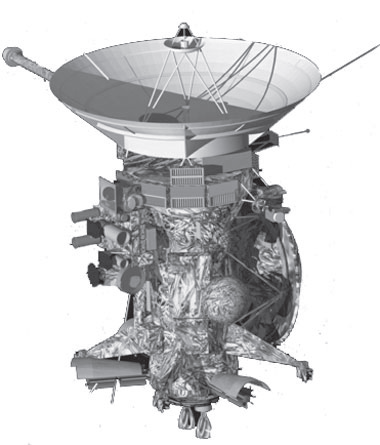
\includegraphics[width=.6\linewidth]{fig_00}
}%figues de la page de garde


\iflivret
\pagestyle{empty}


%%%%%%%% PAGE DE GARDE COURS
\ifcours
% ==== BANDEAU DES TITRES ==== 
\begin{tikzpicture}[remember picture,overlay]
\node at (current page.north west)
{\begin{tikzpicture}[remember picture,overlay]
\node[anchor=north west,inner sep=0pt] at (0,0) {\includegraphics[width=\paperwidth]{\thechapterimage}};
\draw[anchor=west] (-2cm,-8cm) node [line width=2pt,rounded corners=15pt,draw=ocre,fill=white,fill opacity=0.6,inner sep=40pt]{\strut\makebox[22cm]{}};
\draw[anchor=west] (1cm,-8cm) node {\huge\sffamily\bfseries\color{black} %
\begin{minipage}{1cm}
\rotatebox{90}{\LARGE\sffamily\textsc{\color{ocre}\textbf{\xxnumpartie}}}
\end{minipage} \hfill
\begin{minipage}[c]{14cm}
\begin{titrepartie}
\begin{flushright}
\renewcommand{\baselinestretch}{1.1} 
\Large\sffamily\textsc{\textbf{\xxpartie}}
\renewcommand{\baselinestretch}{1} 
\end{flushright}
\end{titrepartie}
\end{minipage} \hfill
\begin{minipage}[c]{3.5cm}
{\large\sffamily\textsc{\textbf{\color{ocre} \discipline}}}
\end{minipage} 
 };
\end{tikzpicture}};
\end{tikzpicture}
% ==== FIN BANDEAU DES TITRES ==== 


% ==== ONGLET 
\begin{tikzpicture}[overlay]
\node[shape=rectangle, 
      rounded corners = .25 cm,
	  draw= ocre,
	  line width=2pt, 
	  fill = ocre!10,
	  minimum width  = 2.5cm,
	  minimum height = 3cm,] at (18.3cm,0) {};
\node at (17.7cm,0) {\rotatebox{90}{\textbf{\Large\color{ocre}{\classe}}}};
%{};
\end{tikzpicture}
% ==== FIN ONGLET 


\vspace{3.5cm}

\begin{tikzpicture}[remember picture,overlay]
\draw[anchor=west] (-2cm,-6cm) node {\huge\sffamily\bfseries\color{black} %
\begin{minipage}{2cm}
\begin{center}
\LARGE\sffamily\textsc{\color{ocre}\textbf{\xxactivite}}
\end{center}
\end{minipage} \hfill
\begin{minipage}[c]{15cm}
\begin{titrechapitre}
\renewcommand{\baselinestretch}{1.1} 
\Large\sffamily\textsc{\textbf{\xxnumchapitre}}

\Large\sffamily\textsc{\textbf{\xxchapitre}}
\vspace{.5cm}

\renewcommand{\baselinestretch}{1} 
\normalsize\normalfont
\xxcompetences
\end{titrechapitre}
\end{minipage}  };
\end{tikzpicture}
\vfill

\begin{flushright}
\begin{minipage}[c]{.3\linewidth}
\begin{center}
\xxfigures
\end{center}
\end{minipage}\hfill
\begin{minipage}[c]{.6\linewidth}
\startcontents
%\printcontents{}{1}{}
\printcontents{}{1}{}
\end{minipage}
\end{flushright}

\begin{tikzpicture}[remember picture,overlay]
\draw[anchor=west] (4.5cm,-.7cm) node {
\begin{minipage}[c]{.2\linewidth}
\begin{flushright}

\includegraphics[width=2cm]{logoCC}
\end{flushright}
\end{minipage}
\begin{minipage}[c]{.2\linewidth}
\textsl{\xxauteur} \\
\textsl{\classe}
\end{minipage}
 };
\end{tikzpicture}

\newpage
\pagestyle{fancy}

%\newpage
%\pagestyle{fancy}

\else
\fi
%% FIN PAGE DE GARDE DES COURS

%%%%%%%% PAGE DE GARDE TD
\iftd
%\begin{tikzpicture}[remember picture,overlay]
%\node at (current page.north west)
%{\begin{tikzpicture}[remember picture,overlay]
%\draw[anchor=west] (-2cm,-3.25cm) node [line width=2pt,rounded corners=15pt,draw=ocre,fill=white,fill opacity=0.6,inner sep=40pt]{\strut\makebox[22cm]{}};
%\draw[anchor=west] (1cm,-3.25cm) node {\huge\sffamily\bfseries\color{black} %
%\begin{minipage}{1cm}
%\rotatebox{90}{\LARGE\sffamily\textsc{\color{ocre}\textbf{\xxnumpartie}}}
%\end{minipage} \hfill
%\begin{minipage}[c]{13.5cm}
%\begin{titrepartie}
%\begin{flushright}
%\renewcommand{\baselinestretch}{1.1} 
%\Large\sffamily\textsc{\textbf{\xxpartie}}
%\renewcommand{\baselinestretch}{1} 
%\end{flushright}
%\end{titrepartie}
%\end{minipage} \hfill
%\begin{minipage}[c]{3.5cm}
%{\large\sffamily\textsc{\textbf{\color{ocre} \discipline}}}
%\end{minipage} 
% };
%\end{tikzpicture}};
%\end{tikzpicture}

%%%%%%%%%% PAGE DE GARDE TD %%%%%%%%%%%%%%%
%\begin{tikzpicture}[overlay]
%\node[shape=rectangle, 
%      rounded corners = .25 cm,
%	  draw= ocre,
%	  line width=2pt, 
%	  fill = ocre!10,
%	  minimum width  = 2.5cm,
%	  minimum height = 2.5cm,] at (18.5cm,0) {};
%\node at (17.7cm,0) {\rotatebox{90}{\textbf{\Large\color{ocre}{\classe}}}};
%%{};
%\end{tikzpicture}

% PARTIE ET CHAPITRE
%\begin{tikzpicture}[remember picture,overlay]
%\draw[anchor=west] (-1cm,-2.1cm) node {\large\sffamily\bfseries\color{black} %
%\begin{minipage}[c]{15cm}
%\begin{flushleft}
%\xxnumchapitre \\
%\xxchapitre
%\end{flushleft}
%\end{minipage}  };
%\end{tikzpicture}

% BANDEAU EXO
\iflivret % SI LIVRET
\begin{tikzpicture}[remember picture,overlay]
\draw[anchor=west] (-2cm,-3.3cm) node {\huge\sffamily\bfseries\color{black} %
\begin{minipage}{5cm}
\begin{center}
\LARGE\sffamily\color{ocre}\textbf{\textsc{\xxactivite}}

\begin{center}
\xxfigures
\end{center}

\end{center}
\end{minipage} \hfill
\begin{minipage}[c]{12cm}
\begin{titrechapitre}
\renewcommand{\baselinestretch}{1.1} 
\large\sffamily\textbf{\textsc{\xxtitreexo}}

\small\sffamily{\textbf{\textit{\color{black!70}\xxsourceexo}}}
\vspace{.5cm}

\renewcommand{\baselinestretch}{1} 
\normalsize\normalfont
\xxcompetences
\end{titrechapitre}
\end{minipage}};
\end{tikzpicture}
\else % ELSE NOT LIVRET
\begin{tikzpicture}[remember picture,overlay]
\draw[anchor=west] (-2cm,-4.5cm) node {\huge\sffamily\bfseries\color{black} %
\begin{minipage}{5cm}
\begin{center}
\LARGE\sffamily\color{ocre}\textbf{\textsc{\xxactivite}}

\begin{center}
\xxfigures
\end{center}

\end{center}
\end{minipage} \hfill
\begin{minipage}[c]{12cm}
\begin{titrechapitre}
\renewcommand{\baselinestretch}{1.1} 
\large\sffamily\textbf{\textsc{\xxtitreexo}}

\small\sffamily{\textbf{\textit{\color{black!70}\xxsourceexo}}}
\vspace{.5cm}

\renewcommand{\baselinestretch}{1} 
\normalsize\normalfont
\xxcompetences
\end{titrechapitre}
\end{minipage}};
\end{tikzpicture}

\fi

\else   % FIN IF TD
\fi


%%%%%%%% PAGE DE GARDE FICHE
\iffiche
\begin{tikzpicture}[remember picture,overlay]
\node at (current page.north west)
{\begin{tikzpicture}[remember picture,overlay]
\draw[anchor=west] (-2cm,-2.25cm) node [line width=2pt,rounded corners=15pt,draw=ocre,fill=white,fill opacity=0.6,inner sep=40pt]{\strut\makebox[22cm]{}};
\draw[anchor=west] (1cm,-2.25cm) node {\huge\sffamily\bfseries\color{black} %
\begin{minipage}{1cm}
\rotatebox{90}{\LARGE\sffamily\textsc{\color{ocre}\textbf{\xxnumpartie}}}
\end{minipage} \hfill
\begin{minipage}[c]{14cm}
\begin{titrepartie}
\begin{flushright}
\renewcommand{\baselinestretch}{1.1} 
\large\sffamily\textsc{\textbf{\xxpartie} \\} 

\vspace{.2cm}

\normalsize\sffamily\textsc{\textbf{\xxnumchapitre -- \xxchapitre}}
\renewcommand{\baselinestretch}{1} 
\end{flushright}
\end{titrepartie}
\end{minipage} \hfill
\begin{minipage}[c]{3.5cm}
{\large\sffamily\textsc{\textbf{\color{ocre} \discipline}}}
\end{minipage} 
 };
\end{tikzpicture}};
\end{tikzpicture}

\iflivret
\begin{tikzpicture}[overlay]
\node[shape=rectangle, 
      rounded corners = .25 cm,
	  draw= ocre,
	  line width=2pt, 
	  fill = ocre!10,
	  minimum width  = 2.5cm,
	  minimum height = 2.5cm,] at (18.5cm,1.1cm) {};
\node at (17.9cm,1.1cm) {\rotatebox{90}{\textsf{\textbf{\large\color{ocre}{\classe}}}}};
%{};
\end{tikzpicture}
\else
\begin{tikzpicture}[overlay]
\node[shape=rectangle, 
      rounded corners = .25 cm,
	  draw= ocre,
	  line width=2pt, 
	  fill = ocre!10,
	  minimum width  = 2.5cm,
%	  minimum height = 2.5cm,] at (18.5cm,1.1cm) {};
	  minimum height = 2.5cm,] at (18.6cm,0cm) {};
\node at (18cm,0cm) {\rotatebox{90}{\textsf{\textbf{\large\color{ocre}{\classe}}}}};
%{};
\end{tikzpicture}

\fi

\else
\fi



\else
\pagestyle{empty}


%%%%%%%% PAGE DE GARDE COURS
\ifcours
% ==== BANDEAU DES TITRES ==== 
\begin{tikzpicture}[remember picture,overlay]
\node at (current page.north west)
{\begin{tikzpicture}[remember picture,overlay]
\node[anchor=north west,inner sep=0pt] at (0,0) {\includegraphics[width=\paperwidth]{\thechapterimage}};
\draw[anchor=west] (-2cm,-8cm) node [line width=2pt,rounded corners=15pt,draw=ocre,fill=white,fill opacity=0.6,inner sep=40pt]{\strut\makebox[22cm]{}};
\draw[anchor=west] (1cm,-8cm) node {\huge\sffamily\bfseries\color{black} %
\begin{minipage}{1cm}
\rotatebox{90}{\LARGE\sffamily\textsc{\color{ocre}\textbf{\xxnumpartie}}}
\end{minipage} \hfill
\begin{minipage}[c]{14cm}
\begin{titrepartie}
\begin{flushright}
\renewcommand{\baselinestretch}{1.1} 
\Large\sffamily\textsc{\textbf{\xxpartie}}
\renewcommand{\baselinestretch}{1} 
\end{flushright}
\end{titrepartie}
\end{minipage} \hfill
\begin{minipage}[c]{3.5cm}
{\large\sffamily\textsc{\textbf{\color{ocre} \discipline}}}
\end{minipage} 
 };
\end{tikzpicture}};
\end{tikzpicture}
% ==== FIN BANDEAU DES TITRES ==== 


% ==== ONGLET 
\begin{tikzpicture}[overlay]
\node[shape=rectangle, 
      rounded corners = .25 cm,
	  draw= ocre,
	  line width=2pt, 
	  fill = ocre!10,
	  minimum width  = 2.5cm,
	  minimum height = 3cm,] at (18.3cm,0) {};
\node at (17.7cm,0) {\rotatebox{90}{\textbf{\Large\color{ocre}{\classe}}}};
%{};
\end{tikzpicture}
% ==== FIN ONGLET 


\vspace{3.5cm}

\begin{tikzpicture}[remember picture,overlay]
\draw[anchor=west] (-2cm,-6cm) node {\huge\sffamily\bfseries\color{black} %
\begin{minipage}{2cm}
\begin{center}
\LARGE\sffamily\textsc{\color{ocre}\textbf{\xxactivite}}
\end{center}
\end{minipage} \hfill
\begin{minipage}[c]{15cm}
\begin{titrechapitre}
\renewcommand{\baselinestretch}{1.1} 
\Large\sffamily\textsc{\textbf{\xxnumchapitre}}

\Large\sffamily\textsc{\textbf{\xxchapitre}}
\vspace{.5cm}

\renewcommand{\baselinestretch}{1} 
\normalsize\normalfont
\xxcompetences
\end{titrechapitre}
\end{minipage}  };
\end{tikzpicture}
\vfill

\begin{flushright}
\begin{minipage}[c]{.3\linewidth}
\begin{center}
\xxfigures
\end{center}
\end{minipage}\hfill
\begin{minipage}[c]{.6\linewidth}
\startcontents
%\printcontents{}{1}{}
\printcontents{}{1}{}
\end{minipage}
\end{flushright}

\begin{tikzpicture}[remember picture,overlay]
\draw[anchor=west] (4.5cm,-.7cm) node {
\begin{minipage}[c]{.2\linewidth}
\begin{flushright}

\includegraphics[width=2cm]{logoCC}
\end{flushright}
\end{minipage}
\begin{minipage}[c]{.2\linewidth}
\textsl{\xxauteur} \\
\textsl{\classe}
\end{minipage}
 };
\end{tikzpicture}

\newpage
\pagestyle{fancy}

%\newpage
%\pagestyle{fancy}

\else
\fi
%% FIN PAGE DE GARDE DES COURS

%%%%%%%% PAGE DE GARDE TD
\iftd
%\begin{tikzpicture}[remember picture,overlay]
%\node at (current page.north west)
%{\begin{tikzpicture}[remember picture,overlay]
%\draw[anchor=west] (-2cm,-3.25cm) node [line width=2pt,rounded corners=15pt,draw=ocre,fill=white,fill opacity=0.6,inner sep=40pt]{\strut\makebox[22cm]{}};
%\draw[anchor=west] (1cm,-3.25cm) node {\huge\sffamily\bfseries\color{black} %
%\begin{minipage}{1cm}
%\rotatebox{90}{\LARGE\sffamily\textsc{\color{ocre}\textbf{\xxnumpartie}}}
%\end{minipage} \hfill
%\begin{minipage}[c]{13.5cm}
%\begin{titrepartie}
%\begin{flushright}
%\renewcommand{\baselinestretch}{1.1} 
%\Large\sffamily\textsc{\textbf{\xxpartie}}
%\renewcommand{\baselinestretch}{1} 
%\end{flushright}
%\end{titrepartie}
%\end{minipage} \hfill
%\begin{minipage}[c]{3.5cm}
%{\large\sffamily\textsc{\textbf{\color{ocre} \discipline}}}
%\end{minipage} 
% };
%\end{tikzpicture}};
%\end{tikzpicture}

%%%%%%%%%% PAGE DE GARDE TD %%%%%%%%%%%%%%%
%\begin{tikzpicture}[overlay]
%\node[shape=rectangle, 
%      rounded corners = .25 cm,
%	  draw= ocre,
%	  line width=2pt, 
%	  fill = ocre!10,
%	  minimum width  = 2.5cm,
%	  minimum height = 2.5cm,] at (18.5cm,0) {};
%\node at (17.7cm,0) {\rotatebox{90}{\textbf{\Large\color{ocre}{\classe}}}};
%%{};
%\end{tikzpicture}

% PARTIE ET CHAPITRE
%\begin{tikzpicture}[remember picture,overlay]
%\draw[anchor=west] (-1cm,-2.1cm) node {\large\sffamily\bfseries\color{black} %
%\begin{minipage}[c]{15cm}
%\begin{flushleft}
%\xxnumchapitre \\
%\xxchapitre
%\end{flushleft}
%\end{minipage}  };
%\end{tikzpicture}

% BANDEAU EXO
\iflivret % SI LIVRET
\begin{tikzpicture}[remember picture,overlay]
\draw[anchor=west] (-2cm,-3.3cm) node {\huge\sffamily\bfseries\color{black} %
\begin{minipage}{5cm}
\begin{center}
\LARGE\sffamily\color{ocre}\textbf{\textsc{\xxactivite}}

\begin{center}
\xxfigures
\end{center}

\end{center}
\end{minipage} \hfill
\begin{minipage}[c]{12cm}
\begin{titrechapitre}
\renewcommand{\baselinestretch}{1.1} 
\large\sffamily\textbf{\textsc{\xxtitreexo}}

\small\sffamily{\textbf{\textit{\color{black!70}\xxsourceexo}}}
\vspace{.5cm}

\renewcommand{\baselinestretch}{1} 
\normalsize\normalfont
\xxcompetences
\end{titrechapitre}
\end{minipage}};
\end{tikzpicture}
\else % ELSE NOT LIVRET
\begin{tikzpicture}[remember picture,overlay]
\draw[anchor=west] (-2cm,-4.5cm) node {\huge\sffamily\bfseries\color{black} %
\begin{minipage}{5cm}
\begin{center}
\LARGE\sffamily\color{ocre}\textbf{\textsc{\xxactivite}}

\begin{center}
\xxfigures
\end{center}

\end{center}
\end{minipage} \hfill
\begin{minipage}[c]{12cm}
\begin{titrechapitre}
\renewcommand{\baselinestretch}{1.1} 
\large\sffamily\textbf{\textsc{\xxtitreexo}}

\small\sffamily{\textbf{\textit{\color{black!70}\xxsourceexo}}}
\vspace{.5cm}

\renewcommand{\baselinestretch}{1} 
\normalsize\normalfont
\xxcompetences
\end{titrechapitre}
\end{minipage}};
\end{tikzpicture}

\fi

\else   % FIN IF TD
\fi


%%%%%%%% PAGE DE GARDE FICHE
\iffiche
\begin{tikzpicture}[remember picture,overlay]
\node at (current page.north west)
{\begin{tikzpicture}[remember picture,overlay]
\draw[anchor=west] (-2cm,-2.25cm) node [line width=2pt,rounded corners=15pt,draw=ocre,fill=white,fill opacity=0.6,inner sep=40pt]{\strut\makebox[22cm]{}};
\draw[anchor=west] (1cm,-2.25cm) node {\huge\sffamily\bfseries\color{black} %
\begin{minipage}{1cm}
\rotatebox{90}{\LARGE\sffamily\textsc{\color{ocre}\textbf{\xxnumpartie}}}
\end{minipage} \hfill
\begin{minipage}[c]{14cm}
\begin{titrepartie}
\begin{flushright}
\renewcommand{\baselinestretch}{1.1} 
\large\sffamily\textsc{\textbf{\xxpartie} \\} 

\vspace{.2cm}

\normalsize\sffamily\textsc{\textbf{\xxnumchapitre -- \xxchapitre}}
\renewcommand{\baselinestretch}{1} 
\end{flushright}
\end{titrepartie}
\end{minipage} \hfill
\begin{minipage}[c]{3.5cm}
{\large\sffamily\textsc{\textbf{\color{ocre} \discipline}}}
\end{minipage} 
 };
\end{tikzpicture}};
\end{tikzpicture}

\iflivret
\begin{tikzpicture}[overlay]
\node[shape=rectangle, 
      rounded corners = .25 cm,
	  draw= ocre,
	  line width=2pt, 
	  fill = ocre!10,
	  minimum width  = 2.5cm,
	  minimum height = 2.5cm,] at (18.5cm,1.1cm) {};
\node at (17.9cm,1.1cm) {\rotatebox{90}{\textsf{\textbf{\large\color{ocre}{\classe}}}}};
%{};
\end{tikzpicture}
\else
\begin{tikzpicture}[overlay]
\node[shape=rectangle, 
      rounded corners = .25 cm,
	  draw= ocre,
	  line width=2pt, 
	  fill = ocre!10,
	  minimum width  = 2.5cm,
%	  minimum height = 2.5cm,] at (18.5cm,1.1cm) {};
	  minimum height = 2.5cm,] at (18.6cm,0cm) {};
\node at (18cm,0cm) {\rotatebox{90}{\textsf{\textbf{\large\color{ocre}{\classe}}}}};
%{};
\end{tikzpicture}

\fi

\else
\fi



\fi
\setlength{\columnseprule}{.1pt}

\pagestyle{fancy}
\thispagestyle{plain}

\ifprof
\vspace{4.5cm}
\else
\vspace{4.5cm}
\fi

\def\columnseprulecolor{\color{ocre}}
\setlength{\columnseprule}{0.4pt} 

%%%%%%%%%%%%%%%%%%%%%%%

\setcounter{exo}{0}

\newcommand{\question}{\textbf{QUESTION}}

\begin{multicols}{2}
\newcommand{\xxexo}{ALG-000}
\section*{algo}
\renewcommand{\xxexo}{ALG-000.tex} 
\subsection*{\xxexo} 
\graphicspath{{../../exos/algo/ALG-000/}}
\input{../../exos/algo/\xxexo} 
 
\renewcommand{\xxexo}{ALG-001.tex} 
\subsection*{\xxexo} 
\graphicspath{{../../exos/algo/ALG-001/}}
\input{../../exos/algo/\xxexo} 
 
\renewcommand{\xxexo}{ALG-002.tex} 
\subsection*{\xxexo} 
\graphicspath{{../../exos/algo/ALG-002/}}
\input{../../exos/algo/\xxexo} 
 
\renewcommand{\xxexo}{ALG-003.tex} 
\subsection*{\xxexo} 
\graphicspath{{../../exos/algo/ALG-003/}}
\input{../../exos/algo/\xxexo} 
 
\renewcommand{\xxexo}{ALG-004.tex} 
\subsection*{\xxexo} 
\graphicspath{{../../exos/algo/ALG-004/}}
\input{../../exos/algo/\xxexo} 
 
\renewcommand{\xxexo}{ALG-005.tex} 
\subsection*{\xxexo} 
\graphicspath{{../../exos/algo/ALG-005/}}
\input{../../exos/algo/\xxexo} 
 
\renewcommand{\xxexo}{ALG-006.tex} 
\subsection*{\xxexo} 
\graphicspath{{../../exos/algo/ALG-006/}}
\input{../../exos/algo/\xxexo} 
 
\renewcommand{\xxexo}{ALG-007.tex} 
\subsection*{\xxexo} 
\graphicspath{{../../exos/algo/ALG-007/}}
\input{../../exos/algo/\xxexo} 
 
\renewcommand{\xxexo}{ALG-008.tex} 
\subsection*{\xxexo} 
\graphicspath{{../../exos/algo/ALG-008/}}
\input{../../exos/algo/\xxexo} 
 
\renewcommand{\xxexo}{ALG-009.tex} 
\subsection*{\xxexo} 
\graphicspath{{../../exos/algo/ALG-009/}}
\input{../../exos/algo/\xxexo} 
 
\renewcommand{\xxexo}{ALG-010.tex} 
\subsection*{\xxexo} 
\graphicspath{{../../exos/algo/ALG-010/}}
\input{../../exos/algo/\xxexo} 
 
\renewcommand{\xxexo}{ALG-011.tex} 
\subsection*{\xxexo} 
\graphicspath{{../../exos/algo/ALG-011/}}
\input{../../exos/algo/\xxexo} 
 
\section*{chaines}
\renewcommand{\xxexo}{STR-000.tex} 
\subsection*{\xxexo} 
\graphicspath{{../../exos/chaines/STR-000/}}
\input{../../exos/chaines/\xxexo} 
 
\renewcommand{\xxexo}{STR-001.tex} 
\subsection*{\xxexo} 
\graphicspath{{../../exos/chaines/STR-001/}}
\input{../../exos/chaines/\xxexo} 
 
\section*{complexite}
\renewcommand{\xxexo}{COM-000.tex} 
\subsection*{\xxexo} 
\graphicspath{{../../exos/complexite/COM-000/}}
\input{../../exos/complexite/\xxexo} 
 
\renewcommand{\xxexo}{COM-001.tex} 
\subsection*{\xxexo} 
\graphicspath{{../../exos/complexite/COM-001/}}
\input{../../exos/complexite/\xxexo} 
 
\renewcommand{\xxexo}{COM-002.tex} 
\subsection*{\xxexo} 
\graphicspath{{../../exos/complexite/COM-002/}}
\input{../../exos/complexite/\xxexo} 
 
\renewcommand{\xxexo}{COM-003.tex} 
\subsection*{\xxexo} 
\graphicspath{{../../exos/complexite/COM-003/}}
\input{../../exos/complexite/\xxexo} 
 
\renewcommand{\xxexo}{COM-004.tex} 
\subsection*{\xxexo} 
\graphicspath{{../../exos/complexite/COM-004/}}
\input{../../exos/complexite/\xxexo} 
 
\renewcommand{\xxexo}{COM-005.tex} 
\subsection*{\xxexo} 
\graphicspath{{../../exos/complexite/COM-005/}}
\input{../../exos/complexite/\xxexo} 
 
\renewcommand{\xxexo}{COM-006.tex} 
\subsection*{\xxexo} 
\graphicspath{{../../exos/complexite/COM-006/}}
\input{../../exos/complexite/\xxexo} 
 
\renewcommand{\xxexo}{COM-007.tex} 
\subsection*{\xxexo} 
\graphicspath{{../../exos/complexite/COM-007/}}
\input{../../exos/complexite/\xxexo} 
 
\section*{equadiffs}
\renewcommand{\xxexo}{EQD-000.tex} 
\subsection*{\xxexo} 
\graphicspath{{../../exos/equadiffs/EQD-000/}}
\input{../../exos/equadiffs/\xxexo} 
 
\renewcommand{\xxexo}{EQD-001.tex} 
\subsection*{\xxexo} 
\graphicspath{{../../exos/equadiffs/EQD-001/}}
\input{../../exos/equadiffs/\xxexo} 
 
\renewcommand{\xxexo}{EQD-002.tex} 
\subsection*{\xxexo} 
\graphicspath{{../../exos/equadiffs/EQD-002/}}
\input{../../exos/equadiffs/\xxexo} 
 
\renewcommand{\xxexo}{EQD-003.tex} 
\subsection*{\xxexo} 
\graphicspath{{../../exos/equadiffs/EQD-003/}}
\input{../../exos/equadiffs/\xxexo} 
 
\section*{fichiers}
\renewcommand{\xxexo}{FIC-000.tex} 
\subsection*{\xxexo} 
\graphicspath{{../../exos/fichiers/FIC-000/}}
\input{../../exos/fichiers/\xxexo} 
 
\renewcommand{\xxexo}{FIC-001.tex} 
\subsection*{\xxexo} 
\graphicspath{{../../exos/fichiers/FIC-001/}}
\input{../../exos/fichiers/\xxexo} 
 
\renewcommand{\xxexo}{FIC-002.tex} 
\subsection*{\xxexo} 
\graphicspath{{../../exos/fichiers/FIC-002/}}
\input{../../exos/fichiers/\xxexo} 
 
\renewcommand{\xxexo}{FIC-003.tex} 
\subsection*{\xxexo} 
\graphicspath{{../../exos/fichiers/FIC-003/}}
\input{../../exos/fichiers/\xxexo} 
 
\renewcommand{\xxexo}{FIC-004.tex} 
\subsection*{\xxexo} 
\graphicspath{{../../exos/fichiers/FIC-004/}}
\input{../../exos/fichiers/\xxexo} 
 
\renewcommand{\xxexo}{FIC-005.tex} 
\subsection*{\xxexo} 
\graphicspath{{../../exos/fichiers/FIC-005/}}
\input{../../exos/fichiers/\xxexo} 
 
\renewcommand{\xxexo}{FIC-006.tex} 
\subsection*{\xxexo} 
\graphicspath{{../../exos/fichiers/FIC-006/}}
\input{../../exos/fichiers/\xxexo} 
 
\renewcommand{\xxexo}{FIC-007.tex} 
\subsection*{\xxexo} 
\graphicspath{{../../exos/fichiers/FIC-007/}}
\input{../../exos/fichiers/\xxexo} 
 
\renewcommand{\xxexo}{FIC-008.tex} 
\subsection*{\xxexo} 
\graphicspath{{../../exos/fichiers/FIC-008/}}
\input{../../exos/fichiers/\xxexo} 
 
\section*{nombres}
\renewcommand{\xxexo}{NBR-000.tex} 
\subsection*{\xxexo} 
\graphicspath{{../../exos/nombres/NBR-000/}}
\input{../../exos/nombres/\xxexo} 
 
\renewcommand{\xxexo}{NBR-001.tex} 
\subsection*{\xxexo} 
\graphicspath{{../../exos/nombres/NBR-001/}}
\input{../../exos/nombres/\xxexo} 
 
\renewcommand{\xxexo}{NBR-002.tex} 
\subsection*{\xxexo} 
\graphicspath{{../../exos/nombres/NBR-002/}}
\input{../../exos/nombres/\xxexo} 
 
\renewcommand{\xxexo}{NBR-003.tex} 
\subsection*{\xxexo} 
\graphicspath{{../../exos/nombres/NBR-003/}}
\input{../../exos/nombres/\xxexo} 
 
\renewcommand{\xxexo}{NBR-004.tex} 
\subsection*{\xxexo} 
\graphicspath{{../../exos/nombres/NBR-004/}}
\input{../../exos/nombres/\xxexo} 
 
\renewcommand{\xxexo}{NBR-005.tex} 
\subsection*{\xxexo} 
\graphicspath{{../../exos/nombres/NBR-005/}}
\input{../../exos/nombres/\xxexo} 
 
\section*{plot}
\renewcommand{\xxexo}{PLT-000.tex} 
\subsection*{\xxexo} 
\graphicspath{{../../exos/plot/PLT-000/}}
\input{../../exos/plot/\xxexo} 
 
\renewcommand{\xxexo}{PLT-001.tex} 
\subsection*{\xxexo} 
\graphicspath{{../../exos/plot/PLT-001/}}
\input{../../exos/plot/\xxexo} 
 
\section*{programmation dynamique}
\renewcommand{\xxexo}{PDY-000.tex} 
\subsection*{\xxexo} 
\graphicspath{{../../exos/programmation_dynamique/PDY-000/}}
\input{../../exos/programmation_dynamique/\xxexo} 
 
\section*{python bases}
\renewcommand{\xxexo}{PYB-000.tex} 
\subsection*{\xxexo} 
\graphicspath{{../../exos/python_bases/PYB-000/}}
\input{../../exos/python_bases/\xxexo} 
 
\renewcommand{\xxexo}{PYB-001.tex} 
\subsection*{\xxexo} 
\graphicspath{{../../exos/python_bases/PYB-001/}}
\input{../../exos/python_bases/\xxexo} 
 
\renewcommand{\xxexo}{PYB-002-bis.tex} 
\subsection*{\xxexo} 
\graphicspath{{../../exos/python_bases/PYB-002-bis/}}
\input{../../exos/python_bases/\xxexo} 
 
\renewcommand{\xxexo}{PYB-002.tex} 
\subsection*{\xxexo} 
\graphicspath{{../../exos/python_bases/PYB-002/}}
\input{../../exos/python_bases/\xxexo} 
 
\renewcommand{\xxexo}{PYB-003-bis.tex} 
\subsection*{\xxexo} 
\graphicspath{{../../exos/python_bases/PYB-003-bis/}}
\input{../../exos/python_bases/\xxexo} 
 
\renewcommand{\xxexo}{PYB-003.tex} 
\subsection*{\xxexo} 
\graphicspath{{../../exos/python_bases/PYB-003/}}
\input{../../exos/python_bases/\xxexo} 
 
\renewcommand{\xxexo}{PYB-004.tex} 
\subsection*{\xxexo} 
\graphicspath{{../../exos/python_bases/PYB-004/}}
\input{../../exos/python_bases/\xxexo} 
 
\renewcommand{\xxexo}{PYB-005.tex} 
\subsection*{\xxexo} 
\graphicspath{{../../exos/python_bases/PYB-005/}}
\input{../../exos/python_bases/\xxexo} 
 
\renewcommand{\xxexo}{PYB-007.tex} 
\subsection*{\xxexo} 
\graphicspath{{../../exos/python_bases/PYB-007/}}
\input{../../exos/python_bases/\xxexo} 
 
\renewcommand{\xxexo}{PYB-100.tex} 
\subsection*{\xxexo} 
\graphicspath{{../../exos/python_bases/PYB-100/}}
\input{../../exos/python_bases/\xxexo} 
 
\renewcommand{\xxexo}{PYB-101.tex} 
\subsection*{\xxexo} 
\graphicspath{{../../exos/python_bases/PYB-101/}}
\input{../../exos/python_bases/\xxexo} 
 
\renewcommand{\xxexo}{PYB-102.tex} 
\subsection*{\xxexo} 
\graphicspath{{../../exos/python_bases/PYB-102/}}
\input{../../exos/python_bases/\xxexo} 
 
\renewcommand{\xxexo}{PYB-103.tex} 
\subsection*{\xxexo} 
\graphicspath{{../../exos/python_bases/PYB-103/}}
\input{../../exos/python_bases/\xxexo} 
 
\renewcommand{\xxexo}{PYB-104.tex} 
\subsection*{\xxexo} 
\graphicspath{{../../exos/python_bases/PYB-104/}}
\input{../../exos/python_bases/\xxexo} 
 
\renewcommand{\xxexo}{PYB-105.tex} 
\subsection*{\xxexo} 
\graphicspath{{../../exos/python_bases/PYB-105/}}
\input{../../exos/python_bases/\xxexo} 
 
\renewcommand{\xxexo}{PYB-106.tex} 
\subsection*{\xxexo} 
\graphicspath{{../../exos/python_bases/PYB-106/}}
\input{../../exos/python_bases/\xxexo} 
 
\renewcommand{\xxexo}{PYB-107.tex} 
\subsection*{\xxexo} 
\graphicspath{{../../exos/python_bases/PYB-107/}}
\input{../../exos/python_bases/\xxexo} 
 
\renewcommand{\xxexo}{PYB-108.tex} 
\subsection*{\xxexo} 
\graphicspath{{../../exos/python_bases/PYB-108/}}
\input{../../exos/python_bases/\xxexo} 
 
\renewcommand{\xxexo}{PYB-109.tex} 
\subsection*{\xxexo} 
\graphicspath{{../../exos/python_bases/PYB-109/}}
\input{../../exos/python_bases/\xxexo} 
 
\renewcommand{\xxexo}{PYB-200.tex} 
\subsection*{\xxexo} 
\graphicspath{{../../exos/python_bases/PYB-200/}}
\input{../../exos/python_bases/\xxexo} 
 
\renewcommand{\xxexo}{PYB-201.tex} 
\subsection*{\xxexo} 
\graphicspath{{../../exos/python_bases/PYB-201/}}
\input{../../exos/python_bases/\xxexo} 
 
\renewcommand{\xxexo}{PYB-202.tex} 
\subsection*{\xxexo} 
\graphicspath{{../../exos/python_bases/PYB-202/}}
\input{../../exos/python_bases/\xxexo} 
 
\renewcommand{\xxexo}{PYB-203.tex} 
\subsection*{\xxexo} 
\graphicspath{{../../exos/python_bases/PYB-203/}}
\input{../../exos/python_bases/\xxexo} 
 
\renewcommand{\xxexo}{PYB-204.tex} 
\subsection*{\xxexo} 
\graphicspath{{../../exos/python_bases/PYB-204/}}
\input{../../exos/python_bases/\xxexo} 
 
\renewcommand{\xxexo}{PYB-205.tex} 
\subsection*{\xxexo} 
\graphicspath{{../../exos/python_bases/PYB-205/}}
\input{../../exos/python_bases/\xxexo} 
 
\renewcommand{\xxexo}{PYB-206.tex} 
\subsection*{\xxexo} 
\graphicspath{{../../exos/python_bases/PYB-206/}}
\input{../../exos/python_bases/\xxexo} 
 
\renewcommand{\xxexo}{PYB-207.tex} 
\subsection*{\xxexo} 
\graphicspath{{../../exos/python_bases/PYB-207/}}
\input{../../exos/python_bases/\xxexo} 
 
\renewcommand{\xxexo}{PYB-208.tex} 
\subsection*{\xxexo} 
\graphicspath{{../../exos/python_bases/PYB-208/}}
\input{../../exos/python_bases/\xxexo} 
 
\renewcommand{\xxexo}{PYB-209.tex} 
\subsection*{\xxexo} 
\graphicspath{{../../exos/python_bases/PYB-209/}}
\input{../../exos/python_bases/\xxexo} 
 
\renewcommand{\xxexo}{PYB-300.tex} 
\subsection*{\xxexo} 
\graphicspath{{../../exos/python_bases/PYB-300/}}
\input{../../exos/python_bases/\xxexo} 
 
\renewcommand{\xxexo}{PYB-301.tex} 
\subsection*{\xxexo} 
\graphicspath{{../../exos/python_bases/PYB-301/}}
\input{../../exos/python_bases/\xxexo} 
 
\renewcommand{\xxexo}{PYB-302.tex} 
\subsection*{\xxexo} 
\graphicspath{{../../exos/python_bases/PYB-302/}}
\input{../../exos/python_bases/\xxexo} 
 
\renewcommand{\xxexo}{PYB-303.tex} 
\subsection*{\xxexo} 
\graphicspath{{../../exos/python_bases/PYB-303/}}
\input{../../exos/python_bases/\xxexo} 
 
\renewcommand{\xxexo}{PYB-304.tex} 
\subsection*{\xxexo} 
\graphicspath{{../../exos/python_bases/PYB-304/}}
\input{../../exos/python_bases/\xxexo} 
 
\renewcommand{\xxexo}{PYB-305.tex} 
\subsection*{\xxexo} 
\graphicspath{{../../exos/python_bases/PYB-305/}}
\input{../../exos/python_bases/\xxexo} 
 
\renewcommand{\xxexo}{PYB-306.tex} 
\subsection*{\xxexo} 
\graphicspath{{../../exos/python_bases/PYB-306/}}
\input{../../exos/python_bases/\xxexo} 
 
\renewcommand{\xxexo}{PYB-307.tex} 
\subsection*{\xxexo} 
\graphicspath{{../../exos/python_bases/PYB-307/}}
\input{../../exos/python_bases/\xxexo} 
 
\renewcommand{\xxexo}{PYB-400.tex} 
\subsection*{\xxexo} 
\graphicspath{{../../exos/python_bases/PYB-400/}}
\input{../../exos/python_bases/\xxexo} 
 
\renewcommand{\xxexo}{PYB-401.tex} 
\subsection*{\xxexo} 
\graphicspath{{../../exos/python_bases/PYB-401/}}
\input{../../exos/python_bases/\xxexo} 
 
\renewcommand{\xxexo}{PYB-402.tex} 
\subsection*{\xxexo} 
\graphicspath{{../../exos/python_bases/PYB-402/}}
\input{../../exos/python_bases/\xxexo} 
 
\renewcommand{\xxexo}{PYB-403.tex} 
\subsection*{\xxexo} 
\graphicspath{{../../exos/python_bases/PYB-403/}}
\input{../../exos/python_bases/\xxexo} 
 
\renewcommand{\xxexo}{PYB-404.tex} 
\subsection*{\xxexo} 
\graphicspath{{../../exos/python_bases/PYB-404/}}
\input{../../exos/python_bases/\xxexo} 
 
\renewcommand{\xxexo}{PYB-405.tex} 
\subsection*{\xxexo} 
\graphicspath{{../../exos/python_bases/PYB-405/}}
\input{../../exos/python_bases/\xxexo} 
 
\renewcommand{\xxexo}{PYB-406.tex} 
\subsection*{\xxexo} 
\graphicspath{{../../exos/python_bases/PYB-406/}}
\input{../../exos/python_bases/\xxexo} 
 
\renewcommand{\xxexo}{PYB-407.tex} 
\subsection*{\xxexo} 
\graphicspath{{../../exos/python_bases/PYB-407/}}
\input{../../exos/python_bases/\xxexo} 
 
\renewcommand{\xxexo}{PYB-408.tex} 
\subsection*{\xxexo} 
\graphicspath{{../../exos/python_bases/PYB-408/}}
\input{../../exos/python_bases/\xxexo} 
 
\renewcommand{\xxexo}{PYB-409.tex} 
\subsection*{\xxexo} 
\graphicspath{{../../exos/python_bases/PYB-409/}}
\input{../../exos/python_bases/\xxexo} 
 
\renewcommand{\xxexo}{PYB-410.tex} 
\subsection*{\xxexo} 
\graphicspath{{../../exos/python_bases/PYB-410/}}
\input{../../exos/python_bases/\xxexo} 
 
\renewcommand{\xxexo}{PYB-500.tex} 
\subsection*{\xxexo} 
\graphicspath{{../../exos/python_bases/PYB-500/}}
\input{../../exos/python_bases/\xxexo} 
 
\renewcommand{\xxexo}{PYB-501.tex} 
\subsection*{\xxexo} 
\graphicspath{{../../exos/python_bases/PYB-501/}}
\input{../../exos/python_bases/\xxexo} 
 
\renewcommand{\xxexo}{PYB-502.tex} 
\subsection*{\xxexo} 
\graphicspath{{../../exos/python_bases/PYB-502/}}
\input{../../exos/python_bases/\xxexo} 
 
\renewcommand{\xxexo}{PYB-503.tex} 
\subsection*{\xxexo} 
\graphicspath{{../../exos/python_bases/PYB-503/}}
\input{../../exos/python_bases/\xxexo} 
 
\renewcommand{\xxexo}{PYB-504.tex} 
\subsection*{\xxexo} 
\graphicspath{{../../exos/python_bases/PYB-504/}}
\input{../../exos/python_bases/\xxexo} 
 
\renewcommand{\xxexo}{PYB-505.tex} 
\subsection*{\xxexo} 
\graphicspath{{../../exos/python_bases/PYB-505/}}
\input{../../exos/python_bases/\xxexo} 
 
\renewcommand{\xxexo}{PYB-506.tex} 
\subsection*{\xxexo} 
\graphicspath{{../../exos/python_bases/PYB-506/}}
\input{../../exos/python_bases/\xxexo} 
 
\renewcommand{\xxexo}{PYB-507.tex} 
\subsection*{\xxexo} 
\graphicspath{{../../exos/python_bases/PYB-507/}}
\input{../../exos/python_bases/\xxexo} 
 
\renewcommand{\xxexo}{PYB-508.tex} 
\subsection*{\xxexo} 
\graphicspath{{../../exos/python_bases/PYB-508/}}
\input{../../exos/python_bases/\xxexo} 
 
\renewcommand{\xxexo}{PYB-509.tex} 
\subsection*{\xxexo} 
\graphicspath{{../../exos/python_bases/PYB-509/}}
\input{../../exos/python_bases/\xxexo} 
 
\renewcommand{\xxexo}{PYB-510.tex} 
\subsection*{\xxexo} 
\graphicspath{{../../exos/python_bases/PYB-510/}}
\input{../../exos/python_bases/\xxexo} 
 
\renewcommand{\xxexo}{PYB-511.tex} 
\subsection*{\xxexo} 
\graphicspath{{../../exos/python_bases/PYB-511/}}
\input{../../exos/python_bases/\xxexo} 
 
\renewcommand{\xxexo}{PYB-512.tex} 
\subsection*{\xxexo} 
\graphicspath{{../../exos/python_bases/PYB-512/}}
\input{../../exos/python_bases/\xxexo} 
 
\renewcommand{\xxexo}{PYB-513.tex} 
\subsection*{\xxexo} 
\graphicspath{{../../exos/python_bases/PYB-513/}}
\input{../../exos/python_bases/\xxexo} 
 
\renewcommand{\xxexo}{PYB-514.tex} 
\subsection*{\xxexo} 
\graphicspath{{../../exos/python_bases/PYB-514/}}
\input{../../exos/python_bases/\xxexo} 
 
\renewcommand{\xxexo}{PYB-515.tex} 
\subsection*{\xxexo} 
\graphicspath{{../../exos/python_bases/PYB-515/}}
\input{../../exos/python_bases/\xxexo} 
 
\renewcommand{\xxexo}{PYB-516.tex} 
\subsection*{\xxexo} 
\graphicspath{{../../exos/python_bases/PYB-516/}}
\input{../../exos/python_bases/\xxexo} 
 
\renewcommand{\xxexo}{PYB-517.tex} 
\subsection*{\xxexo} 
\graphicspath{{../../exos/python_bases/PYB-517/}}
\input{../../exos/python_bases/\xxexo} 
 
\renewcommand{\xxexo}{PYB-518.tex} 
\subsection*{\xxexo} 
\graphicspath{{../../exos/python_bases/PYB-518/}}
\input{../../exos/python_bases/\xxexo} 
 
\section*{sql}
\renewcommand{\xxexo}{SQL-000.tex} 
\subsection*{\xxexo} 
\graphicspath{{../../exos/sql/SQL-000/}}
\input{../../exos/sql/\xxexo} 
 
\renewcommand{\xxexo}{SQL-001.tex} 
\subsection*{\xxexo} 
\graphicspath{{../../exos/sql/SQL-001/}}
\input{../../exos/sql/\xxexo} 
 
\renewcommand{\xxexo}{SQL-002.tex} 
\subsection*{\xxexo} 
\graphicspath{{../../exos/sql/SQL-002/}}
\input{../../exos/sql/\xxexo} 
 
\renewcommand{\xxexo}{SQL-003.tex} 
\subsection*{\xxexo} 
\graphicspath{{../../exos/sql/SQL-003/}}
\input{../../exos/sql/\xxexo} 
 
\section*{systemes}
\renewcommand{\xxexo}{SYS-000.tex} 
\subsection*{\xxexo} 
\graphicspath{{../../exos/systemes/SYS-000/}}
\input{../../exos/systemes/\xxexo} 
 
\renewcommand{\xxexo}{SYS-001.tex} 
\subsection*{\xxexo} 
\graphicspath{{../../exos/systemes/SYS-001/}}
\input{../../exos/systemes/\xxexo} 
 
\renewcommand{\xxexo}{SYS-002.tex} 
\subsection*{\xxexo} 
\graphicspath{{../../exos/systemes/SYS-002/}}
\input{../../exos/systemes/\xxexo} 
 
\section*{tableaux}
\renewcommand{\xxexo}{TAB-000.tex} 
\subsection*{\xxexo} 
\graphicspath{{../../exos/tableaux/TAB-000/}}
\input{../../exos/tableaux/\xxexo} 
 
\renewcommand{\xxexo}{TAB-001.tex} 
\subsection*{\xxexo} 
\graphicspath{{../../exos/tableaux/TAB-001/}}
\input{../../exos/tableaux/\xxexo} 
 
\renewcommand{\xxexo}{TAB-002.tex} 
\subsection*{\xxexo} 
\graphicspath{{../../exos/tableaux/TAB-002/}}
\input{../../exos/tableaux/\xxexo} 
 
\renewcommand{\xxexo}{TAB-003.tex} 
\subsection*{\xxexo} 
\graphicspath{{../../exos/tableaux/TAB-003/}}
\input{../../exos/tableaux/\xxexo} 
 
\renewcommand{\xxexo}{TAB-004.tex} 
\subsection*{\xxexo} 
\graphicspath{{../../exos/tableaux/TAB-004/}}
\input{../../exos/tableaux/\xxexo} 
 
\renewcommand{\xxexo}{TAB-005.tex} 
\subsection*{\xxexo} 
\graphicspath{{../../exos/tableaux/TAB-005/}}
\input{../../exos/tableaux/\xxexo} 
 
\renewcommand{\xxexo}{TAB-006.tex} 
\subsection*{\xxexo} 
\graphicspath{{../../exos/tableaux/TAB-006/}}
\input{../../exos/tableaux/\xxexo} 
 
\renewcommand{\xxexo}{TAB-007.tex} 
\subsection*{\xxexo} 
\graphicspath{{../../exos/tableaux/TAB-007/}}
\input{../../exos/tableaux/\xxexo} 
 
\renewcommand{\xxexo}{TAB-008.tex} 
\subsection*{\xxexo} 
\graphicspath{{../../exos/tableaux/TAB-008/}}
\input{../../exos/tableaux/\xxexo} 
 
\renewcommand{\xxexo}{TAB-009.tex} 
\subsection*{\xxexo} 
\graphicspath{{../../exos/tableaux/TAB-009/}}
\input{../../exos/tableaux/\xxexo} 
 
\renewcommand{\xxexo}{TAB-010.tex} 
\subsection*{\xxexo} 
\graphicspath{{../../exos/tableaux/TAB-010/}}
\input{../../exos/tableaux/\xxexo} 
 
\renewcommand{\xxexo}{TAB-011.tex} 
\subsection*{\xxexo} 
\graphicspath{{../../exos/tableaux/TAB-011/}}
\input{../../exos/tableaux/\xxexo} 
 
\renewcommand{\xxexo}{TAB-012.tex} 
\subsection*{\xxexo} 
\graphicspath{{../../exos/tableaux/TAB-012/}}
\input{../../exos/tableaux/\xxexo} 
 
\renewcommand{\xxexo}{TAB-013.tex} 
\subsection*{\xxexo} 
\graphicspath{{../../exos/tableaux/TAB-013/}}
\input{../../exos/tableaux/\xxexo} 
 
\renewcommand{\xxexo}{TAB-014.tex} 
\subsection*{\xxexo} 
\graphicspath{{../../exos/tableaux/TAB-014/}}
\input{../../exos/tableaux/\xxexo} 
 
\renewcommand{\xxexo}{TAB-015.tex} 
\subsection*{\xxexo} 
\graphicspath{{../../exos/tableaux/TAB-015/}}
\input{../../exos/tableaux/\xxexo} 
 
\renewcommand{\xxexo}{TAB-016.tex} 
\subsection*{\xxexo} 
\graphicspath{{../../exos/tableaux/TAB-016/}}
\input{../../exos/tableaux/\xxexo} 
 
\renewcommand{\xxexo}{TAB-017.tex} 
\subsection*{\xxexo} 
\graphicspath{{../../exos/tableaux/TAB-017/}}
\input{../../exos/tableaux/\xxexo} 
 
\renewcommand{\xxexo}{TAB-018.tex} 
\subsection*{\xxexo} 
\graphicspath{{../../exos/tableaux/TAB-018/}}
\input{../../exos/tableaux/\xxexo} 
 
\renewcommand{\xxexo}{TAB-019.tex} 
\subsection*{\xxexo} 
\graphicspath{{../../exos/tableaux/TAB-019/}}
\input{../../exos/tableaux/\xxexo} 
 
\renewcommand{\xxexo}{TAB-020.tex} 
\subsection*{\xxexo} 
\graphicspath{{../../exos/tableaux/TAB-020/}}
\input{../../exos/tableaux/\xxexo} 
 
\renewcommand{\xxexo}{TAB-021.tex} 
\subsection*{\xxexo} 
\graphicspath{{../../exos/tableaux/TAB-021/}}
\input{../../exos/tableaux/\xxexo} 
 
\renewcommand{\xxexo}{TAB-022.tex} 
\subsection*{\xxexo} 
\graphicspath{{../../exos/tableaux/TAB-022/}}
\input{../../exos/tableaux/\xxexo} 
 
\renewcommand{\xxexo}{TAB-023.tex} 
\subsection*{\xxexo} 
\graphicspath{{../../exos/tableaux/TAB-023/}}
\input{../../exos/tableaux/\xxexo} 
 


%\renewcommand{\xxexo}{COM-002} 
%\subsection*{\xxexo} 
%\graphicspath{{../../exos/complexite/COM-002/}}
%\input{../../exos/complexite/\xxexo} 

\end{multicols}

